\documentclass[compress]{beamer}


\usepackage[utf8]{inputenc}
\usepackage[T1]{fontenc}

\usepackage{dwlecture}


\title{Dyna 2009}

\author{Dawid Weiss}
\institute{Institute of Computing Science\\Poznan University of Technology}

\date{}

\AtBeginSection[] {
  \begin{frame}<beamer>
    \framesubtitle{\insertpart}
    \tableofcontents[sectionstyle=show/shaded,subsectionstyle=show/shaded/hide]
  \end{frame}
}

\AtBeginSubsection[] {
  \begin{frame}<beamer>
    \framesubtitle{\insertpart}
    \tableofcontents[sectionstyle=shaded,subsectionstyle=show/shaded/hide]
  \end{frame}
}

\begin{document}

\begin{frame}[plain,fragile,t]
    \begin{center}
    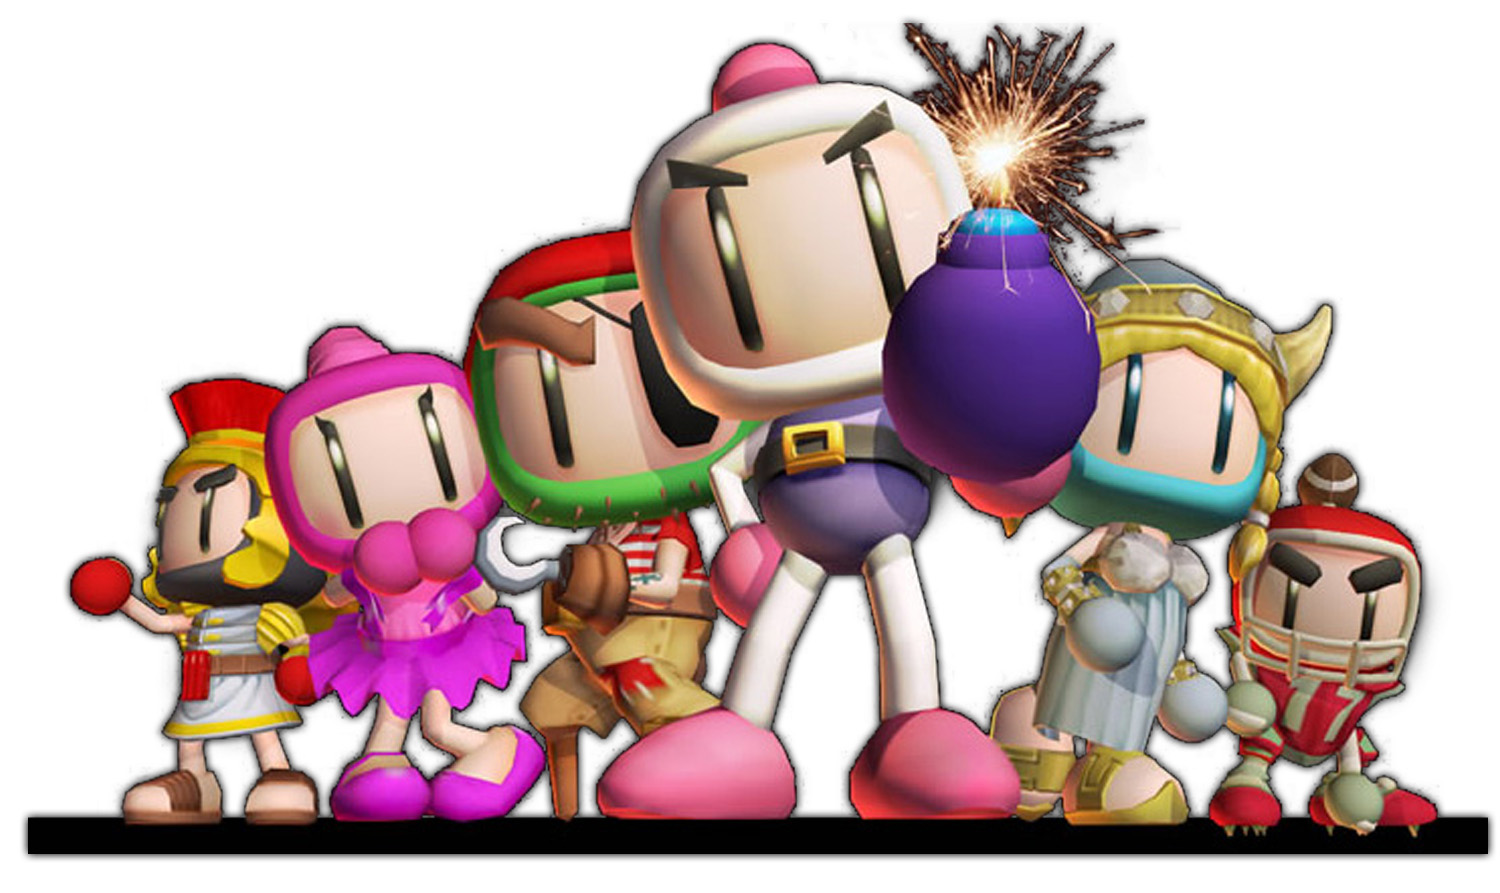
\includegraphics[width=.9\linewidth]{figures/dyna}\\[2mm]
    \textbl{DYNA BLASTER}\\
    Technologie Wytwarzania Oprogramowania '2009
    \end{center}
    \pplogo
\end{frame}

\begin{frame}[plain]
    \begin{center}
    \textbl{DYNA BLASTER}
    \end{center}
\end{frame}

\begin{frame}[plain]
    \hgraphics{figures/screen1}
\end{frame}

\begin{frame}[plain]    
    \vgraphics{figures/screen2}
\end{frame}

\begin{frame}[plain]
    \begin{abscenter}
    \textbl{CEL ZADANIA}
    \end{abscenter}
\end{frame}

\begin{frame}[plain]
    \begin{abscenter}
        \only<1>{
\includegraphics[height=8cm]{figures/corba} }
        \only<2>{
\includegraphics[height=8cm]{figures/smith} }
        \only<3>{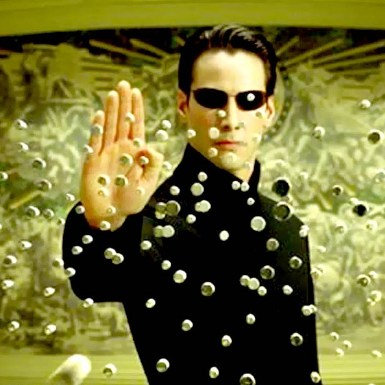
\includegraphics[height=8cm]{figures/neo} }
        \only<4>{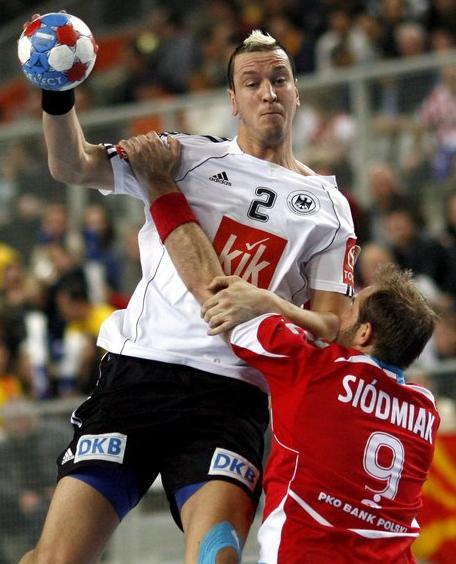
\includegraphics[height=8cm]{figures/siodmiakzhensem} }
        \only<5>{%
            
\includegraphics[height=3cm]{figures/corba}
            
\includegraphics[height=3cm]{figures/smith}
            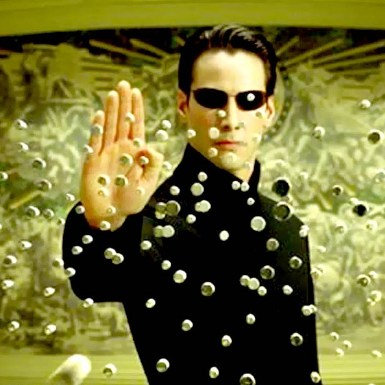
\includegraphics[height=3cm]{figures/neo}}
    \end{abscenter}
    
    \only<5>{
        \begin{center}
        CORBA + AGENCI + LUDZIE
        \end{center}
    }
\end{frame}

\begin{frame}[plain]
    \begin{abscenter}
    \textbl{API}
    \end{abscenter}
\end{frame}

\begin{frame}[plain, fragile]
    \begin{javablock}[numbers=none]
public interface IPlayerController
{
    enum Direction
    {
        LEFT, RIGHT, UP, DOWN
    }

    public Direction getCurrent();

    public boolean dropsBomb();
}
    \end{javablock}
    
    \bigskip
    \begin{center}
    ASYNC CALLS. 25 FPS. 
    \end{center}
\end{frame}

\begin{frame}[plain]
    \vgraphics{figures/vulture}
\end{frame}

\begin{frame}[plain]
    \begin{center}
    ROZGRYWKA I\\[1cm]
    \textbl{BOTY}\\[1cm]
    \end{center}
\end{frame}

\begin{frame}[plain]
    \textbl{Reguły}
    
    \bigskip
    \begin{itemize}
        \item System pucharowy.
        \item Liczba żyć: 3.
        \item Max 3 minuty na całość.
        \item Plansza: tournament-2
        \item Cel: \emph{there may be only one}.

        \bigskip\color{gray}
        \item Bomb: 2, Zakres: 3, Bonusy. 
    \end{itemize}
\end{frame}

\begin{frame}[plain,fragile]
    \begin{itemize}
        \item \texttt{http://192.168.0.XXX:8080/dyna-webapp/jdyna.zip}
        \item Rozpakować.
        \item Uruchomić konsolę (bash lub cmd).
        \item Bot musi być spakowany do JARa i nazwany \texttt{player.jar}.
    \end{itemize}
\end{frame}

\begin{frame}[plain,fragile]
    \begin{screenblock}[fontsize=\Large, numbers=none]
jdyna bot --no-view --no-sound 
  -n MYNAME -g GAMEROOM package.ClassName
    \end{screenblock}
\end{frame}


\begin{frame}[plain]
    \begin{center}
    ROZGRYWKA II\\[1cm]
    \textbl{WIELE BOTÓW}\\[1cm]
    \end{center}
\end{frame}

\begin{frame}[plain]
    \hgraphics{figures/wszyscy}
\end{frame}

\begin{frame}[plain]
    \textbl{Reguły}
    
    \bigskip
    \begin{itemize}
        \item Wszyscy na planszy od razu.
        \item Liczba żyć: 5.
        \item Max 5 minut na całość.
        \item Plansza: (1) bigclassic
        \item Plansza: (2) tournament-3
        \item Cele: \emph{mass-killer}, \emph{dodger}.

        \bigskip\color{gray}
        \item Bomb: 2, Zakres: 3, Bonusy. 
    \end{itemize}
\end{frame}


\begin{frame}[plain]
    \begin{center}
    ROZGRYWKA III\\[1cm]
    \textbl{BOTY vs. LUDZIE}\\[1cm]
    \end{center}
\end{frame}

\begin{frame}[plain]
    \begin{center}
    \only<+>{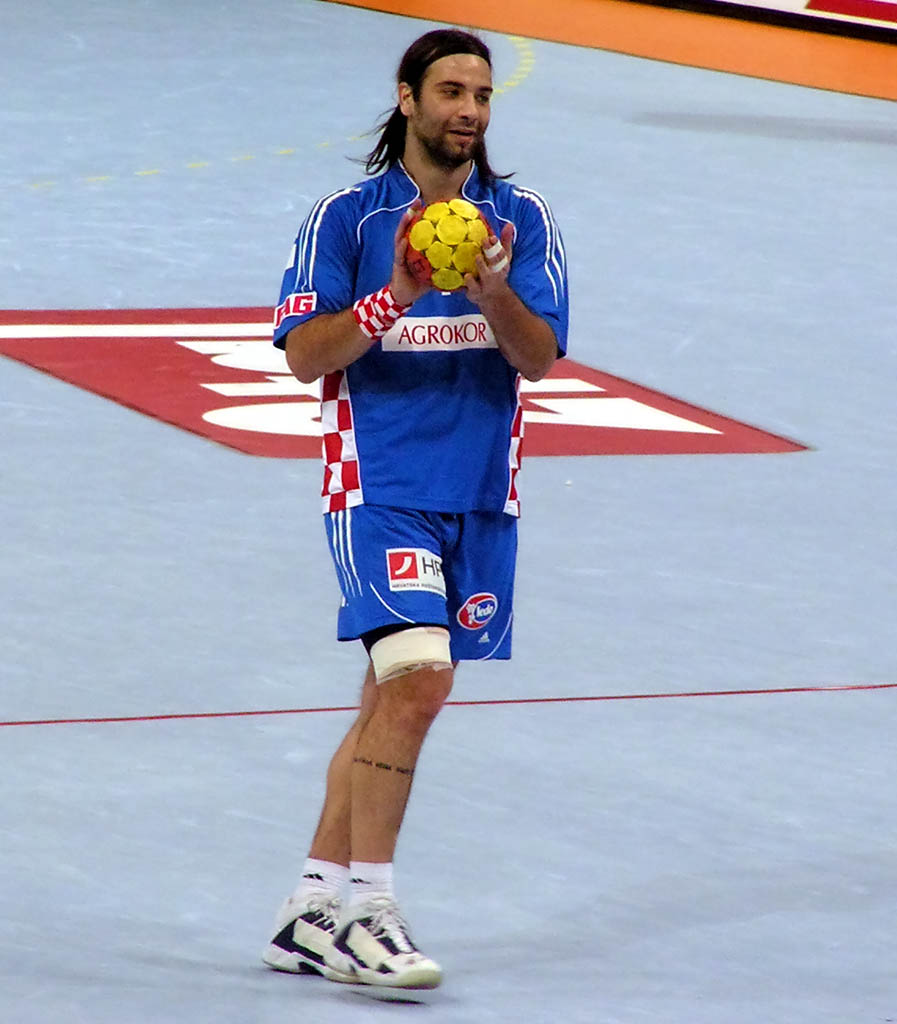
\includegraphics[height=8cm]{figures/balic}}
    \only<+>{\hgraphics{figures/siodmiak}}
    \end{center}
\end{frame}

\begin{frame}[plain]
    \textbl{Reguły}
    
    \bigskip
    \begin{itemize}
        \item DWIE DRUŻYNY!
        \item Liczba żyć: 5.
        \item Max 5 minut na całość.
        \item Plansza: (1) bigclassic
        \item Cel: \emph{ZACIUKAĆ BOTY}

        \bigskip\color{gray}
        \item Bomb: 2, Zakres: 3, Bonusy. 
    \end{itemize}
\end{frame}

\begin{frame}[plain,fragile]
    \begin{itemize}
        \item \texttt{http://192.168.0.XXX:8080/dyna-webapp/jdyna.zip}
        \item Rozpakować.
        \item Uruchomić konsolę (bash lub cmd).
    \end{itemize}
\end{frame}

\begin{frame}[plain,fragile]
    Ludzie:
    \begin{screenblock}[fontsize=\Large, numbers=none]
jdyna human --no-view --no-sound 
       -n "human:MYNAME" -g GAMEROOM
    \end{screenblock}

    \bigskip
    Boty:
    \begin{screenblock}[fontsize=\Large, numbers=none]
jdyna bot --no-view --no-sound 
       -n "bot:MYNAME" -g GAMEROOM 
           package.ClassName
    \end{screenblock}    
\end{frame}

\begin{frame}[plain]
    \begin{center}
    http://jdyna.com/
    \end{center}
\end{frame}

\end{document}
